\documentclass[12pt]{article}

\usepackage{graphicx}
\usepackage{color}   %May be necessary if you want to color links
\usepackage{hyperref}
\hypersetup{
    colorlinks=true, %set true if you want colored links
    linktoc=all,     %set to all if you want both sections and subsections linked
    linkcolor=blue,  %choose some color if you want links to stand out
}

\usepackage{textcomp}

%puts figure captions on the bottom
\usepackage{floatrow}
\floatsetup[figure]{capposition=bottom}

%verbatim stuff
\usepackage{fancyvrb}


%step enumaration
\usepackage{enumitem}
\newlist{steps}{enumerate}{1}
\setlist[steps, 1]{label = \textbf{Step \arabic*:}}

%page break after sections
\usepackage{titlesec}
\newcommand{\sectionbreak}{\clearpage}

%remove indentation at Paragraph and add line break
\setlength{\parindent}{0em}
\setlength{\parskip}{1em}

\title{MineBike Game Documentation}
\author{Andrew Weller \& [your name here]}
\date{July 2019}

\setcounter{section}{-1}


\begin{document}
\maketitle

\tableofcontents

\section{This Manual}
Hello anonymous developer! Welcome to the MineBike project. If this is not your desired destination you may leave this document now.

If you are not already aware of what the project is, mineBike is a minecraft mod designed as an alternative to traditional physical therapy for quarantined hospital patients who are unable to go outside to excercise. 

Please refer to the table of contents if you wish to find what you are looking for quickly. Otherwise reading this manual in chronological order should get you up to speed with the game with zero prior knowledge.

\subsection{What is this manual?}

This manual is intended to inform the user about the mineBike GAME portion of the code. This manual does not relate to the middleware or the database portion.
If you are looking for documentation on that, you should search elsewhere. 

HOWEVER, there will be a section explaining (not as well as the rest of the manual) where to begin searching to find out about how the game receives information from the bike's raspberry pi.

\subsection {What will this manual teach you?}

If you want to add {\bfseries CONTENT} to the MineBike game, this is the right place to be. This manual will go over all the tools you need to add your own minigames/quests to this game.

If you have other goals in mind this manual will still be valuable as it will show you the important parts of the code so that you can search for pieces relevant to your goal.

\section {Setup}
Setting the game up on your computer is \emph {relatively} painless. If you have set up minecraft forge before this is a bonus, because it is pretty much the exact same process with a slight twist for this mod's specific quirks.



\begin{steps}
  \item Install Java JDK 8.

	  Minecraft was written over 10 years ago and still depends on Java 8 to build. Go to \href {https://www.oracle.com/technetwork/java/javase/downloads/jdk8-downloads-2133151.html} {this download page} and select the latest Java 8 JDK for your operating system.

  \item Install Minecraft Forge

	  Go to \href {https://files.minecraftforge.net/maven/net/minecraftforge/forge/index\_1.7.10.html} {the minecraft forge downloads page for minecraft 1.7.10} and download the Installer if you are on mac/linux or the windows installer if you are on windows.

  \item Clone Repository
		\begin{verbatim}
				$ git clone https://github.com/andrewwellercs/mineBikeCopy
		\end{verbatim}

  \item Unzip Forge Source

		Unzip "MinecraftMod/Forge Source/forge-1.7.10-10.13.4.1492-1.7.10-src.zip" into "MinecraftMod/".

		Be sure to overwrite any files.

		Your MinecraftMod/ directory should look like this now:
		\begin{figure}[H]
			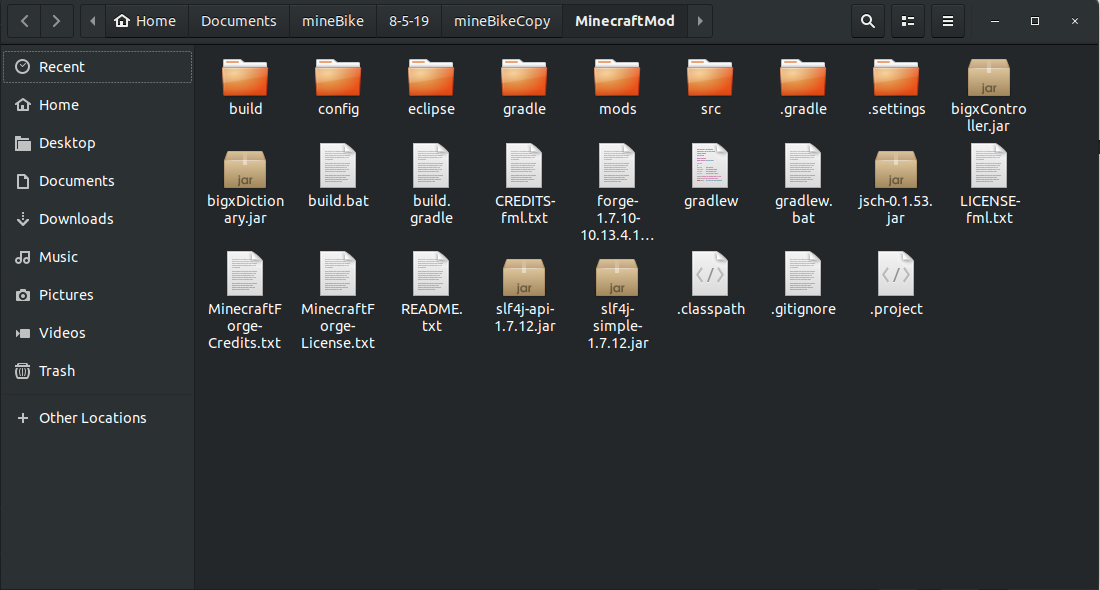
\includegraphics[scale=0.2]{images/setup/MinecraftModDirectory.png}
			\centering
		\end{figure}



  \item Run gradle scripts

	  After unzipping all that stuff there should be a script called gradlew inside of the MinecraftMod/ directory. Run the script using these commands in either your terminal or command prompt.

		Mac/Linux (terminal):
	\begin{verbatim}
		$ ./gradlew setupDecompWorkspace --refresh-dependencies
		
		$ ./gradlew eclipse
	\end{verbatim}

		Windows (command prompt):

	\begin{verbatim}
		$ gradlew.bat setupDecompWorkspace --refresh-dependencies
		
		$ gradlew.bat eclipse
	\end{verbatim}

	This will create an eclipse workspace in the MinecraftMod/ directory.

  \item Import into Eclipse

	  Go to File $\rightarrow$ Import in eclipse.

	\begin{figure}[H]
		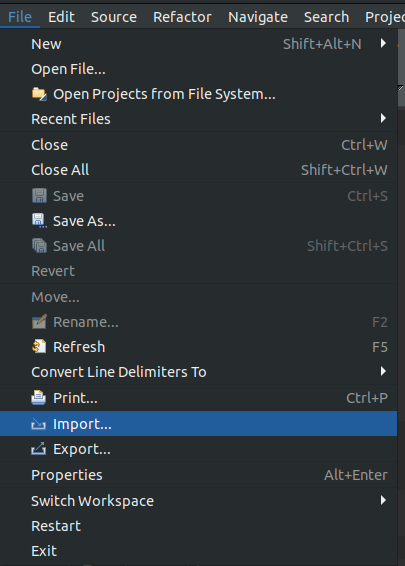
\includegraphics[scale=0.3]{images/setup/FileImport.png}
		\centering
	\end{figure}


	  Then go to General $\rightarrow$ Existing Projects into Workspace (remember the gradlew scripts created the workspace).

	\begin{figure}[H]
		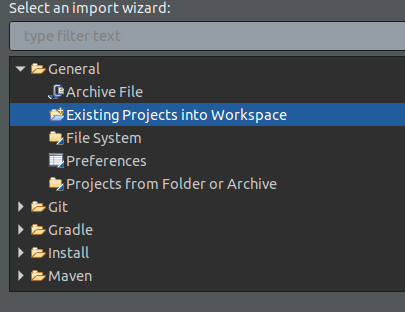
\includegraphics[scale=0.5]{images/setup/GeneralExisting.png}
		\centering
	\end{figure}

	Next for the root directory point eclipse to the location that the MinecraftMod/ folder in your copy of the repository.

	\begin{figure}[H]
		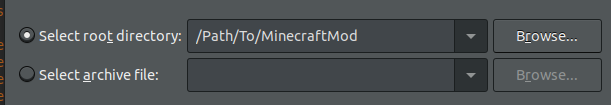
\includegraphics[scale=0.5]{images/setup/ImportDirectory.png}
		\centering
	\end{figure}


  \item Final setup instructions for eclipse.

	  Now there are a couple things you need to do before eclipse will be able to launch the project.

	  First, you have to link some jars that are included with the project.

	  Go to Project $\rightarrow$ Properties in eclipse.

	\begin{figure}[H]
		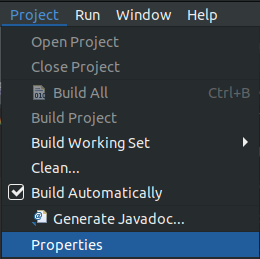
\includegraphics[scale=0.5]{images/setup/ProjectProperties.png}
		\centering
	\end{figure}


	  Then go to Java Build Path $\rightarrow$ Libraries tab $\rightarrow$ Add Jars.

	\begin{figure}[H]
		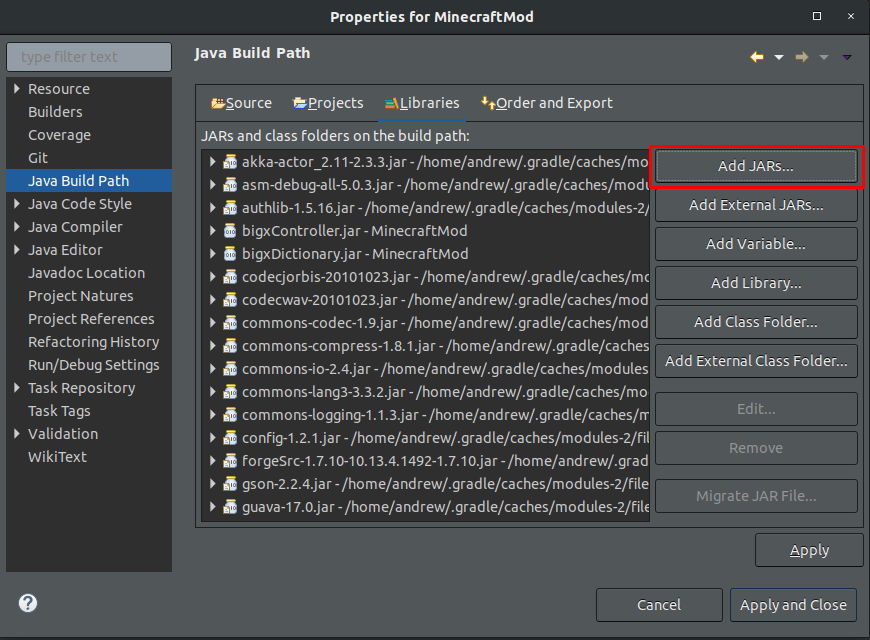
\includegraphics[scale=0.3]{images/setup/AddJars.png}
		\centering
	\end{figure}

	Select bigxController.jar, bigxDictionary.jar, jsch-0.1.53.jar, and slf4j-simple-1.7.12.jar. (slf4j-api-1.7.12.jar is not required, I don't know why, please edit this document if you figure out why)

	\begin{figure}[H]
		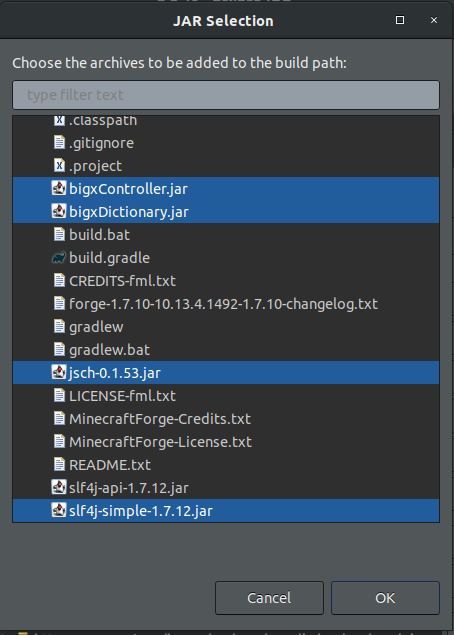
\includegraphics[scale=0.3]{images/setup/WhichJars.png}
		\centering
	\end{figure}

  \item Launching the Game.

	  You're almost done. You might have noticed that if you try to launch the project that it doesn't work. You need to point eclipse towards the main class so that it can start the game properly.

	  You can do this by going to Run $\rightarrow$ Run Configurations, then double click Java Application.

	  This will create a new run configuration.
	  
	  Now click search in the main class box, and then find GradleStart.

	\begin{figure}[H]
		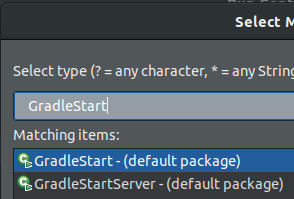
\includegraphics[scale=0.6]{images/setup/GradleStart.png}
		\centering
	\end{figure}

	Now when you run it, it should work. 

	The first time you run the application, you will receive a pop-up that looks like this.

	\begin{figure}[H]
		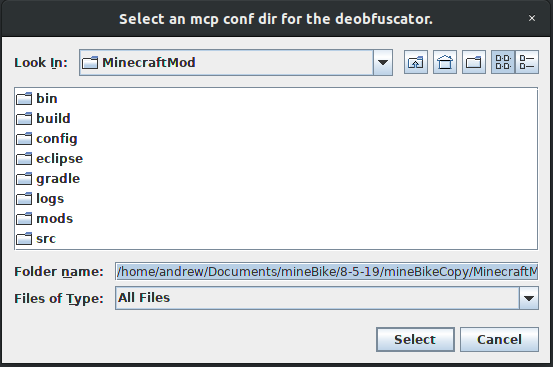
\includegraphics[scale=0.5]{images/setup/PopUp.png}
		\centering
	\end{figure}


\end{steps}

\section {Codebase Overview}
\label{sec:overview}
\begin{figure}[H]
	
\includegraphics[scale=0.5]{images/will_smith_with_camera}
	\centering
\end{figure}
The Codebase looks very big, but there are only a few very important parts to it. Most of the code is either not necessary for manipulating the game or is deprecated. Let's take a look at some important packages. 

\subsection{org.ngs.bigx.minecraft.npcs}
\begin{figure}[H]
	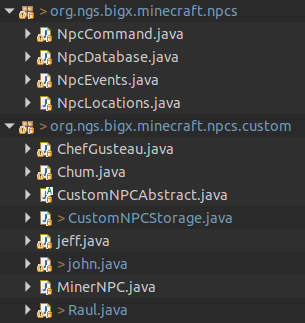
\includegraphics[scale=0.5]{images/tour/orgNgsBigxMinecraftNpcs.png}
	\centering
\end{figure}

This package is largely responsible for the creation of NPCs in the overworld map. Creating npcs in quests is another story and you can learn about it in \hyperref[sec:npcs]{the npcs section}. 

Noteable classes in here include {\bfseries CustomNpcAbstract} which combined with a simple addition to {\bfseries CustomNpcStorage} is a one-stop shop to adding simple npcs into the game. More on that in \hyperref[sec:npcs]{the npcs section}.

\subsection{org.ngs.bigx.minecraft.quests(.custom)}
\begin{figure}[H]
	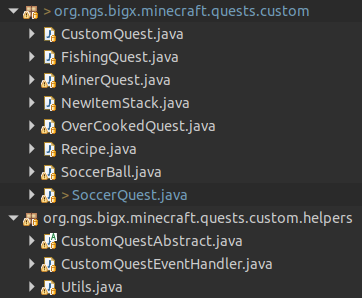
\includegraphics[scale=0.5]{images/tour/orgNgsBigxMinecraftQuestsCustom.png}
	\centering
\end{figure}

This package is responsible for the "quests" or "minigames" that the game has, excluding the original ChasingQuest which was in the game. The questing system is a modular way to build minigames.

\subsection{org.ngs.bigx.minecraft.client.gui.hud}
\begin{figure}[H]
	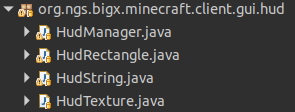
\includegraphics[scale=0.5]{images/tour/orgNgsBigxMinecraftClientGuiHud.png}
	\centering
\end{figure}

This package is very short and specialized. The tools in here can be used to add HUD elements to the game with no knowledge of OpenGL.

More on the usage of this package can be found in the \hyperref[sec:hud]{Hud section}.

\section{Npcs}
\label{sec:npcs}

You might wonder why npcs are first in this guide and not quests. The answer is simple. Npcs are easier to add to the game. So to get your feet wet it is recommended to do this first. Also every quest usually has an npc attached to it. That is the pattern for this game. You start quests by talking to npcs. So once you have created your own npc you can then attach a quest to them and start testing that in the next section.

\subsection{Simple Npcs (overworld)}

Adding Npcs to the overworld is easy.
\begin{figure}[H]
	\caption{A custom NPC made using the CustomNpcAbstract class}
	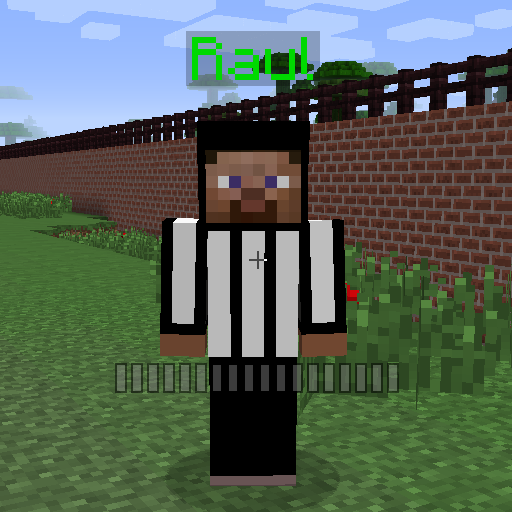
\includegraphics[scale=0.5]{images/npcs/Raul.png}
	\centering
\end{figure}

You can add your own npc by creating a new class the extends the class {\bfseries CustomNpcAbstract}. Located in the package {\bfseries org.ngs.bigx.minecraft.npcs.custom}.

\begin{figure}[H]
	\caption{The CustomNpcAbstract class}
	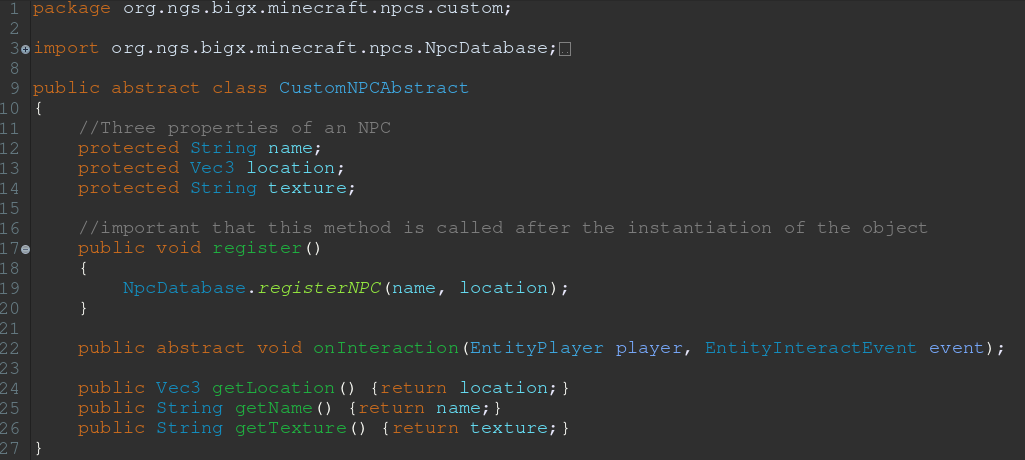
\includegraphics[scale=0.5]{images/npcs/CustomNpcAbstract.png}
	\centering
\end{figure}

There are three protected variables inside this class that should be set in the constructor in order for this class to work as intended. 

\begin{verbatim}
		protected String name;
\end{verbatim}

This variable will change the display name of the npc in game. It is also used as an identifier in other pieces of the code so it should be {\bfseries unique} and not overlap with any other npcs that exist either in the {\bfseries CustomNPCStorage} class or the {\bfseries NpcDatabase} class, located in org.ngs.bigx.minecraft.npcs.custom and org.ngs.bigx.minecraft.npcs packages respectively.

\begin{verbatim}
	protected Vec3 location;	
\end{verbatim}

This variable will change the location that the npc spawns at in the overworld. It should be created with the Vec3.createVectorHelper method.

\begin{verbatim}
		protected String texture;
\end{verbatim}

This variable will change the texture that the npc has in the game. It should be a file location of an image. It technically shouldn't matter where the image is located but sometimes it doesn't work if the images is in a weird folder. In order to guarantee that it works it should be located somewhere in the src/main/resources/assets/customnpcs/ folders, by convention all the skins for customnpcs have been placed inside of the .../customnpcs/textures/entity/ folders

The variable must be set in a certain way. In order to set the texture to a texture in customnpcs/textures/entity/humanmale/ the texture variable should be set as follows: \begin{verbatim} customnpcs:textures/entity/humanmale/Example_Texture.png \end{verbatim}

You can find new textures online by searching for "minecraft skins" online. Note that you will have to find one that is in the right format for the version of the game this mod is using - 1.7.10.

Here is an example of an Npc made using this formula. You can also view this in the project as Raul.java in org.ngs.bigx.minecraft.npcs.custom

\begin{figure}[H]
	\caption{An example of an npc made with the CustomNpcAbstract}
	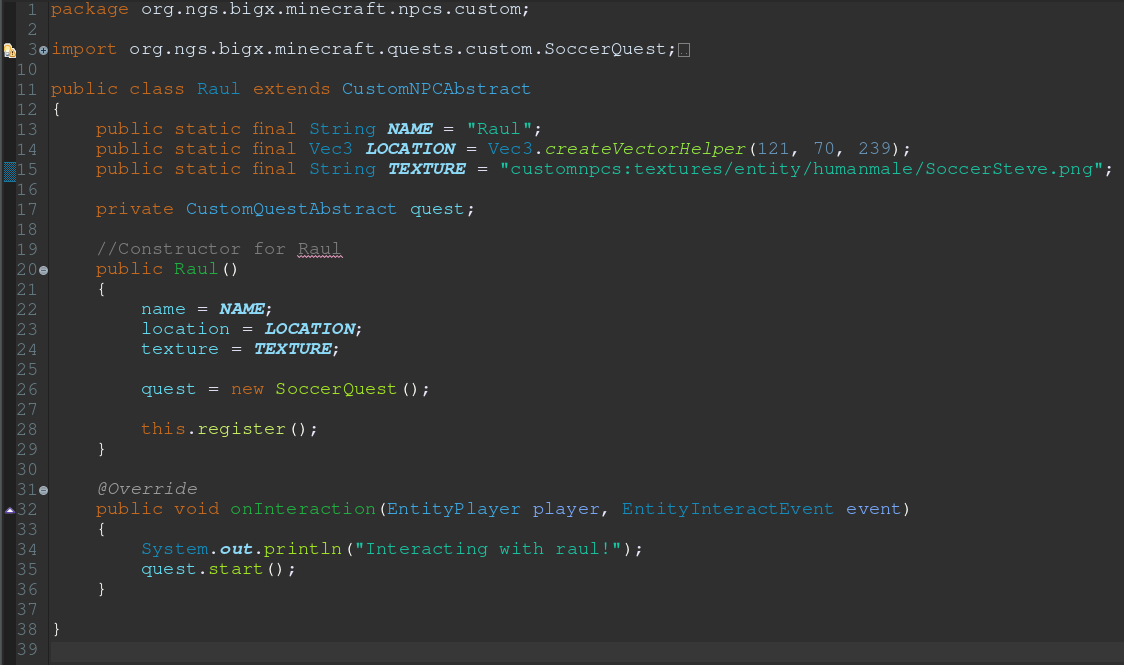
\includegraphics[scale=0.3]{images/npcs/Raul_Java.png}
	\centering
\end{figure}

\subsection{Advanced Npcs (quests/moving)}

If you wish to add an Npc that {\emph does \emph something} into the game, continue reading.

\section{Quests}
\label{sec:quests}

\subsection{What is a quest?}
A quest in the mineBike game is basically just a class that has access to the Minecraft forge event bus. So if a quest is active you can run certain code when different events happen in the game. 

\subsection{Making a quest}

To make a quest, much like an npc you must create a new class which extends the class {\bfseries CustomQuestAbstract} (org.ngs.bigx.minecraft.quests.custom.helpers)

Inside this class there are several methods which correspond to different minecraft forge events. All you have to do is override those methods to make your class do stuff. If you look at the code inside of the class {\bfseries CustomQuestEventHandler} it will become apparent what is going on here.

Let's take a look at the class and what each of the methods does.

\begin{figure}[H]
	\caption{The CustomQuestAbstract class}
	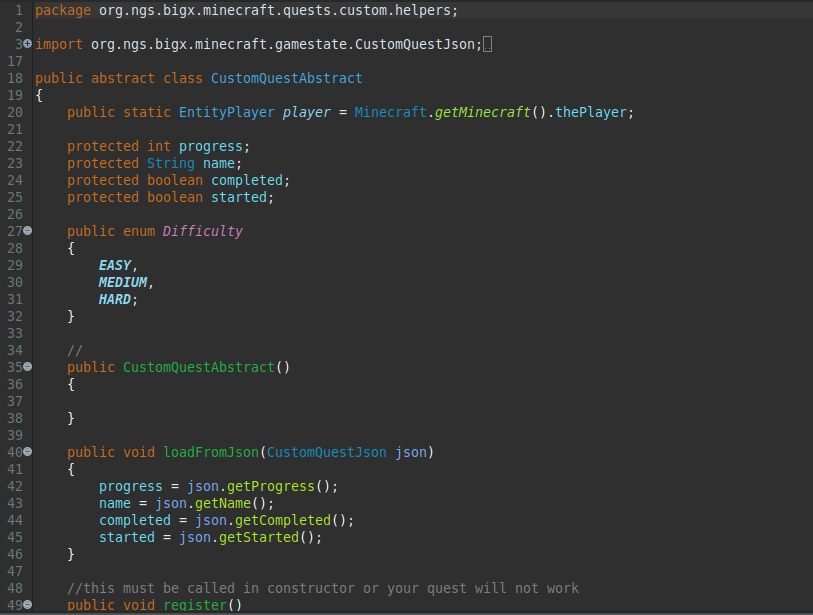
\includegraphics[scale=0.3]{images/quests/CustomQuestAbstract.png}
	\centering
\end{figure}

Foreword: Most of this information is available online, I would start searching here

\subsubsection{onPlayerTickEvent \& onWorldTickEvent}

These two methods are very similar so they will both be talked about in this section. These methods are fired continuously by the game's event bus. If you've played minecraft before, you might know that minecraft's game engine runs at 20 ticks per second. This does not apply here. Yes the game runs at 20 ticks per second, but that means that {\emph one single object} in the game receives an update 20 times a second. This method is a catch all, such that every time a single object is updated, this method is called. There is a a science to the madness but basically you can think of these methods as something that gets executed every frame or just on a loop, however they cannot be reliably used to count time. 

The only reason you would use one over the other is that the onWorldTickEvent's parameter (TickEvent.WorldTickEvent) allows you to access the {\emph world} object from the game and the onPlayerTickEvent's parameter (TickEvent.PlayerTickEvent) allows you to access the {\emph player} object which is being ticked.

Note: When acessing a world from a world tick event, it is useful to make sure that you are accessing one that has both been loaded and that you are accessing the right dimension.

\subsubsection{onItemUse}

This method is called whenever the player right clicks with an item in their hand that does something on right click. This may come in handy for you.

\subsubsection{onItemPickUp}

This method is called whenever the player picks up an item off the ground or is given one from a call of the /give command inside the game. You might find this useful to check when a player is picking up gold etc.

Personally a lot of previous developers have used this as a debugging mechanism to end the quest.

\subsubsection{onAttackEntityEvent}

This method is called whenever an entity is attacked. It grants you access to the entities involved in the transaction.

\subsubsection{onEntityInteractEvent}

Called whenever the player right clicks on an entity who is interactable (a villager, etc.) Grants access to the parties of the transaction.

\subsubsection{onWorldLoadEvent}

This one is important. It is called whenever the player loads into a new dimension. So if the player was transported into a new dimension for a quest to start, this method should be used to verify that the dimension has been loaded before trying to modify the world of that dimension. You can see this pattern in a couple of the quests that already exist where the quest sets a worldLoaded flag in this event.

\subsubsection{onEntityJoinWorld}

Called whenever an entity changes dimensions. Similar to the previous method, but don't use this for that same purpose.

\subsubsection{onQuit}

Called when the game is exited.


\subsection{Making it work}
In order for the quest to actually do stuff it must be registered with the CustomQuestEventHandler. You can do this by calling {\bfseries CustomQuestEventHandler.registerQuest(CustomQuestAbstract quest)} and remove it with {\bfseries unregisterQuest}.

The event methods of the CustomQuestAbstract class sit dormant until the quest has been registered with the CustomQuestEventHandler. A look at the {\bfseries CustomQuestEventHandler} class will illuminate how this works. Then they will start being called appropriately. This effectively keeps track of the "active" quest, and you could perhaps have multiple quests going on at the same time. This has not yet been done though in the game.

The CustomQuestEventHandler is just a regular minecraft forge event handler. You can learn more about it here \url{https://mcforge.readthedocs.io/en/latest/events/intro/}

The easiest way to go about getting your quest to start normally is to attach your quest to an Npc made with the {\bfseries CustomNPCAbstract} class. You can see examples of this by looking at npcs that already exist like {\bfseries Raul}.

\begin{figure}[H]
	\caption{Raul, who has a SoccerQuest as a private data member.}
	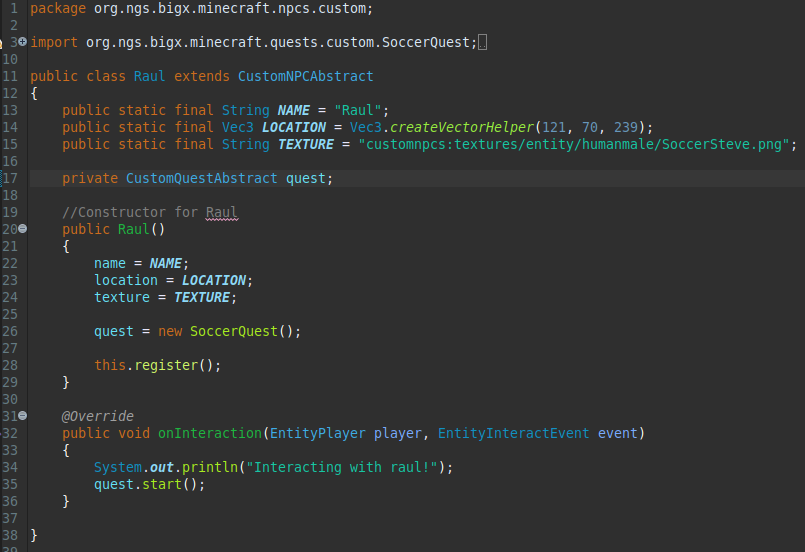
\includegraphics[scale=0.3]{images/quests/RaulQuest.png}
	\centering
\end{figure}

When the npc is interacted with, it calls the {\bfseries start()} method in the CustomQuestAbstract class. By default this method registers the class with the event handler, so that after the quest is started, all of its methods will start being called from the forge event bus.


\section{Hud}
\label{sec:hud}

\end{document}

